\chapter{D\'emarche de conception effectu\'ee}
\label{chap:outils utilises}

\section{Utilisation du gestionnaire de version }
\subsection{Pr\'esentation}
\index{gestionnaire de version}
La r\'ealisation de notre projet informatique a en premier lieu n\'ecessit\'e la mise en place d'une interface centralisant tous nos
documents en temps r\'eel. Pour cela nous avons utilis\'e ce que l'on appelle un gestionnaire de version. Plusieurs logiciels de gestions 
de versions existent aujourd'hui : CVS, Subversion, Mercurial, Bazar et enfin Git\cite{git}, ayant chacun leurs avantages et inconv\'enients. 

Ils permettent d'archiver et de conserver les diff\'erentes \'etapes de d\'eveloppement d'un projet. Ainsi il est possible de pouvoir revenir
\`a une version ant\'erieure \`a tout moment. Ils permettent \'egalement de visualiser les diff\'erences entre les r\'evisions. Cela permet un  
travail collaboratif tr\`es efficace : chaque d\'eveloppeur dispose du projet en local et peut quand il le souhaite les partager sur un serveur.

Nous avons utilis\'e pour notre projet\citep{projet11efr}, le logiciel Git.

\subsection{Le logiciel Git}
\index{git@Git}
Git est un logiciel libre cr\'ee par Linus Torvalds, le fondateur de Linux. C'est un logiciel de version distribu\'e c'est \`a dire qu'il n'est
 pas n\'ecessaire d'utiliser un serveur pour partager nos documents : on peut chacun se synchroniser entre nous.

Au premier abord l'utilisation de git n'est pas \'evidente : toutes les manipulations se font \`a travers la console et le vocabulaire utilis\'e 
est totalement nouveau. 

Apr\`es l'installation de git, il est n\'ecessaire de s'enregistrer (mail et nom) et de cr\'eer un dossier de travail dans lequel nous 
initialisons git en utilisant la commande
\begin{verbatim} git init \end{verbatim}
Ce dossier de travail sera le d\'ep\^ot de notre projet informatique. L'ajout d'un fichier dans le dossier reconnu par git s'effectue en tapant
\begin{verbatim} git add <nom du fichier> \end{verbatim}
La commande
\begin{verbatim} git commit <nom du fichier> \end{verbatim} permet d'enregistrer la modification effectu\'ee dans le dossier de travail.
Ces deux commandes furent utilis\'ees maintes fois lors de notre projet. 

Cependant tout cela reste local : il faut mettre \`a jour le git en utilisant
\begin{verbatim} git push \end{verbatim}
pour rajouter dans le dossier racine, contenant tous le travail des diff\'erents membres du projet, nos nouveaux fichiers. 
De m\^eme, pour t\'el\'echarger ce qui fut r\'ealis\'e par les autres membres du projet nous avons utilis\'e la commande
\begin{verbatim} git pull \end{verbatim}

Enfin, comme chaque membre du groupe peut modifier et am\'eliorer les fichiers en local, il est n\'ecessaire d'ajouter cette branche locale \`a la branche
principale du projet en << fusionnant >> les deux branches :
\begin{verbatim} git merge <nom de la branche>\end{verbatim}
Nous constatons sur la figure \ref{fig:branche} que cette op\'eration a \'et\'e effectu\'ee mainte fois lors de notre travail.

\begin{figure}[h]
\begin{center}
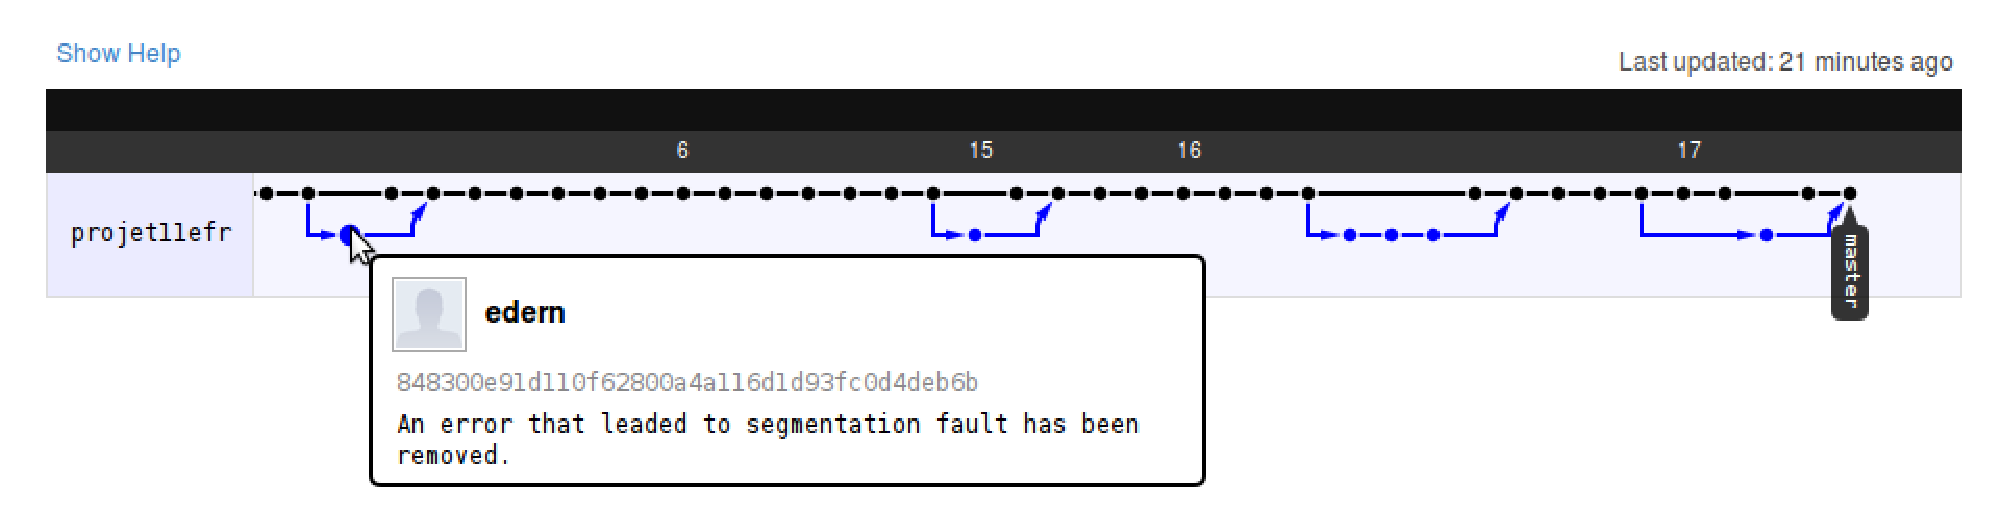
\includegraphics[width=16cm]{branche.eps}
\end{center}
\caption{Modifications effetu\'ees sur la branche principale (master, en noir) du projet par << fusion >> de la branche locale (en bleu)}
\label{fig:branche}
\end{figure}

Ceci constituent les commandes de bases utilis\'es lors de notre projet. Une fois le principe assimil\'e git devient tr\`es simple d'utilisation,
 tr\`es rapide mais surtout tr\`es efficace.

Enfin une des particularit\'es de Git est l'existence de sites web collaboratifs bas\'es sur Git comme Github ou Gitorious. 

\subsection{Github}

Github peut \^etre consid\'er\'e comme un r\'eseau social pour les programmeurs. En effet c'est un << entrep\^ot >> de projet utilisant git comme 
gestionnaire de version. Ainsi Github permet \`a un quelconque utilisateur d'intervenir dans un projet , d'utiliser ces codes sources etc.
GitHub cr\'ee une page de profil simple o\`u appara\^it notre nom, email, etc. Cette page affiche \'egalement notre activit\'e (commit, ajout de suivi,...)
 et nos d\'ep\^ots. De m\^eme nous pouvons recevoir si on le souhaite les mise \`a  jour ( commit, comment) li\'es \`a un projet quelconque.

Les pages d'un projet commencent par une s\'erie d'onglets permettant de parcourir les sources (page par d\'efaut), d'acc\'eder \`a la liste des
 commits, le network, les demandes de pull, les probl\`emes et les wikis.
La page source, qui est la plus importante, contient toute l'arborescence de notre projet, l'adresse SSH et HTTP et permet une vue simple
 de l'avancement de notre travail.
Les autres pages furent moins utilis\'ees car secondaire. 

Cette collaboration entre Git et Github a \'et\'e essentielle pour notre projet et a permis un suivi clair et pr\'ecis de son avancement.

\section{Automatisation de la compilation de notre projet}
\subsection{Compilation avec des Makefiles}

La compilation d'un fichier s'effectue en langage C s'effectue de la mani\`ere suivante :
\begin{verbatim} gcc -c numaverage.c\end{verbatim}
\begin{verbatim} gcc -o numaverage numaverage.o\end{verbatim}

La premi\`ere \'etape correspondant \`a la transformation en code binaire, la seconde \`a l'\'edition des liens.

Pour chaque ex\'ecutable, \`a chaque modification du code source, il faut \'ecrire ces quelques lignes dans un terminal.
Nous avons donc utilis\'e le Makefile pour compiler notre code (cf. figure \ref{fig:exemple_makefile}), afin d'automatiser cett \'etape.
En effet, la commande << \textbf{make} >> cr\'ee l'ex\'ecutable de tous les fichiers cod\'es en langage C d\'efinis dans le makefile. La commande
<< \textbf{make clean} >> supprime tous les fichiers temporaires.
\newline
\begin{figure}[h] 
\begin{center}

\begin{minipage}[|c|]{0.7\linewidth}
\begin{verbatim}
  UTILS = numaverage numbound
  CC = gcc CFlAGS = -WALL
  LIBS = -lm
  all : $(UTILS).o
    for util in $(UTILS) ; do \
      $$(CC) $(CFLAGS) -o $$util $$util.o ; done

  $(UTILS).o:
    for util in $(UTILS) ; do \
      $$(CC) $(CFLAGS) -c $$util.c ; done

  clean :
    $(RM) $(EXEC).o
\end{verbatim}
\end{minipage}
\end{center}
\caption{Syntaxe d'un de nos premiers Makefile}
\label{fig:exemple_makefile}
\end{figure}

Toutefois, l'\'ecriture manuelle d'un Makefile devient impossible si l'on veut ult\'erieurement cr\'eer un paquet debian.
En effet, le principal probl\`eme de ce type de Makefile est qu'il est identique pour chaque syst\`eme d'exploitation. Or certains fichiers
syst\`emes sont n\'ecessaires pour l'utilisation de notre biblioth\`equ num-utils-ng, mais ils ne sont pas forc\'ement dans le r\'epertoire pour
chaqu syst\`eme d'exploitation.
\newline 	
Par cons\'equent, il nous a \'et\'e propos\'e d'utiliser des \textbf{autotools} pour cr\'eer des Makefiles << dynamiques >>, qui d\'ependent du syst\`eme
d'exploitation de l'utlisateur.

\subsection{G\'en\'eration automatique de Makefiles : utilisation des autotools}

L'utilisation d'autotools n\'ecessite de suivre une d\'emarche sp\'ecifique afin de cr\'eer nos Makefiles. Nous avons utilis\'e pour
cela trois outils : automake\citep{automake}, autoconf\citep{tuto_autotool} et aclocal, des logiciels open source, disponibles sur les serveurs debian.
\begin{figure}[h]
 \centerline{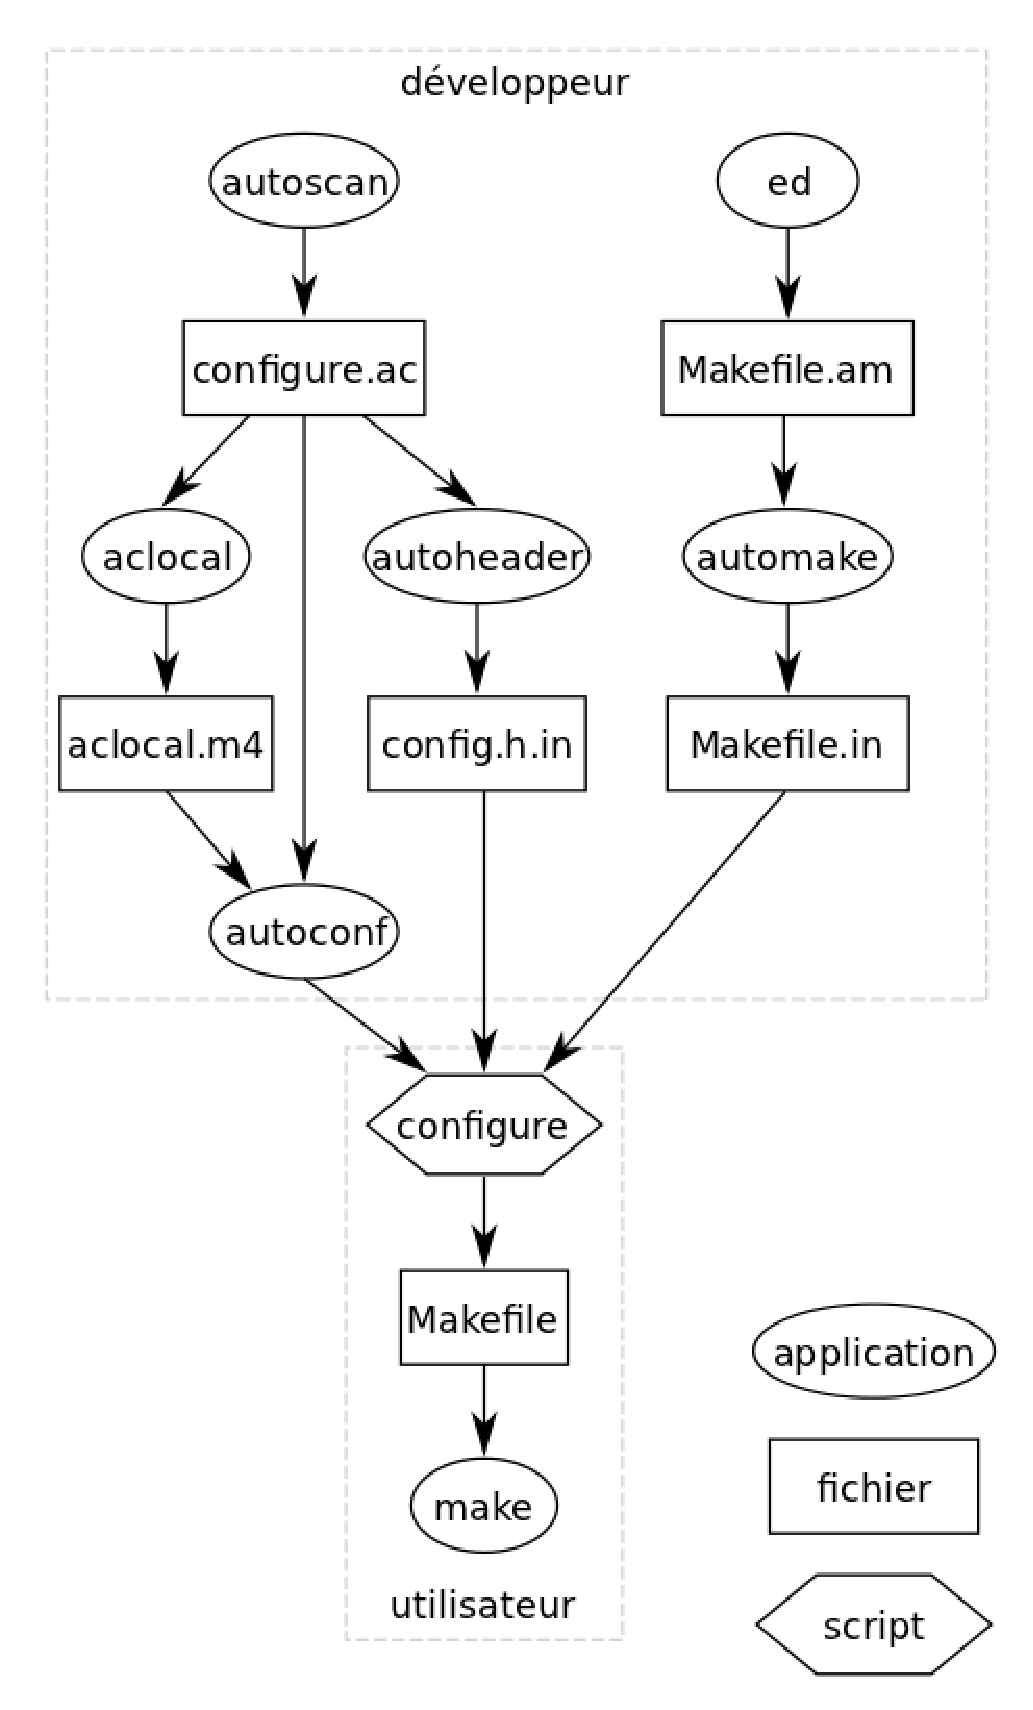
\includegraphics[width=0.45\textwidth]{autotool.eps}}
\caption{\'Etapes n\'ecessaires pour obtenir un Makefile avec un autotools (source : Wikip\'edia)} \label{fig:autotool}
\end{figure}
Le sch\'ema \ref{fig:autotool} illustre les diff\'erentes \'etapes que nous avons suivies pour obtenir les Makefiles.
Nous constatons qu'un certain nombre de fichiers est g\'en\'er\'e lors de l'ex\'ecution des diff\'erents programmes.
Nous allons d\'etailler le r\^ole de ces principaux fichiers :
\newline
\begin{itemize}
 \item [\textbullet] \textbf{ configure.ac :} Le fichier configure.ac est g\'en\'er\'e lors de l'ex\'cution de la commande << autoscan >>
qui va ajouter l'ensemble des macros n\'ecessaires pour autoconf. C'est ce fichier qui permet de r\'esoudre les probl\^emes de portabilit\'e du code.
\newline
 \item [\textbullet] \textbf{ Makefile.am :} Le fichier Makefile.am contient ce que l'ancien Makefile << statique >> contenait sauf que la syntaxe est 
plus simple et plus efficace (il existe notamment de nombreuses variables pr\'ed\'efinies comme << bin\_DIRS >> ou << man\_MANS >> qui permettent l'installation
dans le bon r\'epertoire des ex\'ecutables ou des pages du manuel).  
\newline
\newline
\textbf{Remarque importante} : un des avantages des autotools est que le d\'eveloppeur a peu de texte \`a \'ecrire. Nous avons seulement eu \`a \'ecrire dans
deux fichiers : configure.ac et dans chaque fichier Makefile.am. Tous les autres fichiers on \'et\'e g\'en\'er\'e.
\newline
\end{itemize}
Une fois ces deux \'etapes effectu\'es, il ne nous reste plus qu'\`a g\'en\'erer les diff\'erents fichiers de configuration \`a l'aide des commandes :
\begin{itemize}
 \item [-] \textbf{aclocal} : g\'en\'ere le fichier << aclocal.m4 >> contenant les macros n\'ecessaires pour automake,
 \item [-] \textbf{autoconf} : produit une premi\`ere version du fichier << configure >> (on utilisera \`a nouveau cette commande apr\`es avoir ex\'ecut\'e 
la commande << automake >>, afin de mettre de nouveau \`a jour le fichier << configure >>.
Remarque : nous n'avons pas eu besoin  d'utiliser la commande << autoheader >> car nous n'avions pas de variables de pr\'e-processeur dans notre code.
 \item [-] \textbf{automake} : produit les fichiers Makefile.in (Makefile interm\'ediaire qui seront utilis\'es par le fichier << configure >>.
\newline
\end{itemize}
Ainsi, tout utilisateur peut utiliser notre biblioth\`eque en ex\'cutant le script :
\begin{verbatim}./configure\end{verbatim}
pour cr\'eer les Makefiles dans les diff\'rents r\'epertoire de notre projet.
Le tableau \ref{tab:commandes} montre les principales commandes qui peuvent maintenant \^etre ex\'ecut\'ees :
\begin{table}[h]
\begin{center}

\begin{tabular}{|l|c|r|}
  \hline
  Commande &  Action\\
  \hline
  \textbf{make ou make all} & Cr\'eer les ex\'ecutables \\
  \textbf{make clean} & Supprimer les fichiers cr\'ees\\
  \textbf{make check} & Effectuer une s\'erie de tests \\
  \textbf{make install} & Installer la bibliot\`eque \\
  \textbf{make uninstall} & D\'esintaller la biblioth\`eque \\
  \textbf{make dist} & Cr\'eer une archive de notre projet \\
  \hline
\end{tabular}
\caption{Principales commandes d'un makefile}
\end{center}
\label{tab:commandes}
\end{table}

\section{Cr\'eation du paquet debian}

L'ultime \'etape de notre projet de conception a \'et\`e la cr\'eation du paquet Debian de la biblioth\`eque num-utils-ng.
Sa cr\'eation n\'ecessite de suivre une d\'marche rigoureuse et sp\'ecifique, notamment si nous voulons le publier notre paquet afin
qu'il apparaisse plus tard dans les d\'ep\^ots Debian.
\newline
Premi\`erement, il nous a fallu cr\'eer un repertoire << /debian >> contenant plusieurs fichiers de configuration :
\begin{itemize}
 \item [-] \textbf{rules} : ce fichier inclut les r\`egles qui vont servir pour compiler notre paquet,
 \item [-] \textbf{control} : control contient les d\'ependences du paquet (CDBS et debhelper pour nous),
 \item [-] \textbf{changelog} : changelog contient la liste des diff\'rentes versions du paquet, 
 \item [-] \textbf{copyright} : ce fichier pr\'cise la licence sous laquelle est publi\'e le paquet (GNU General Public License version 3).
Tous ces fichiers sont n\'ecessaires lors  de la cr\'eation d'un paquet Debian. Toutefois, nous avons utilis\'e le logiciel 
CDBS, Common Debian Build System\citep{cdbs} qui permet de simplifier l'\'etape de cr\'eation du paquet et d'\'ecriture des fichiers de configuration.
\newline
\end{itemize}
Une fois le dossier /debian compl\`et\'e, il reste \`a compiler le paquet avec la commande
\begin{verbatim}debuild -us -uc\end{verbatim}
afin de cr\'eer une archive ayant l'extension \textbf{.deb}, notre paquet binaire Debian.
\newline
Remarque importante : L'\'etape de cr\'ation du paquet binaire .deb s'est faite sur une ordinateur fonctionnant avec Ubuntu. Il nous a fallu utiliser le logiciel pbuilder. Ce logiciel
permet de << simuler >> l'\'etat du syst\`eme d'exploitation juste apr\`es son installation (on cr\'ee un environnement isol\'e, appel\'e chroot en anglais).
Ainsi, on peut v\'erifier que toutes les d\'ependances de notre paquet sont bien d\'finies dans le fichier << control >>, 
\newline

Tout utilisateur d'un syst\`eme Unix peut maintenant installer notre paquet num-utils-ng en utilisant dpkg, le syst\`eme de gestion de paquets Debian 
par defaut en tapant :
\begin{verbatim}dpkg -i num-utils-ng_1.0-1_i386.deb\end{verbatim}
La version du paquet \'etant la 1.0-1.





